\subsection{Verification of the Velocity Model}
In the former section a simplified first order model of the vehicle's velocity model was established. To ensure the approximation is a reliable model of the system, it is compared to a measured step-response of the vehicle. However, the simulation uses a first order model as described in the previous section, the gain, found in \appref{app:gainTest} and the time constant, found in \appref{app:inertiaTest}, is used as the first orders parameters. In \figref{SimulationIRLsteprespons2} the simulated model's step-response and the measured step-response of the vehicle is illustrated. 
%
\begin{figure}[H]
  \centering
 	%Trim margins @:   left        bottom       right       top
 	\adjustbox{ trim = {.15\width} {.30\height} {.15\width} {.30\height}, clip }
  {
    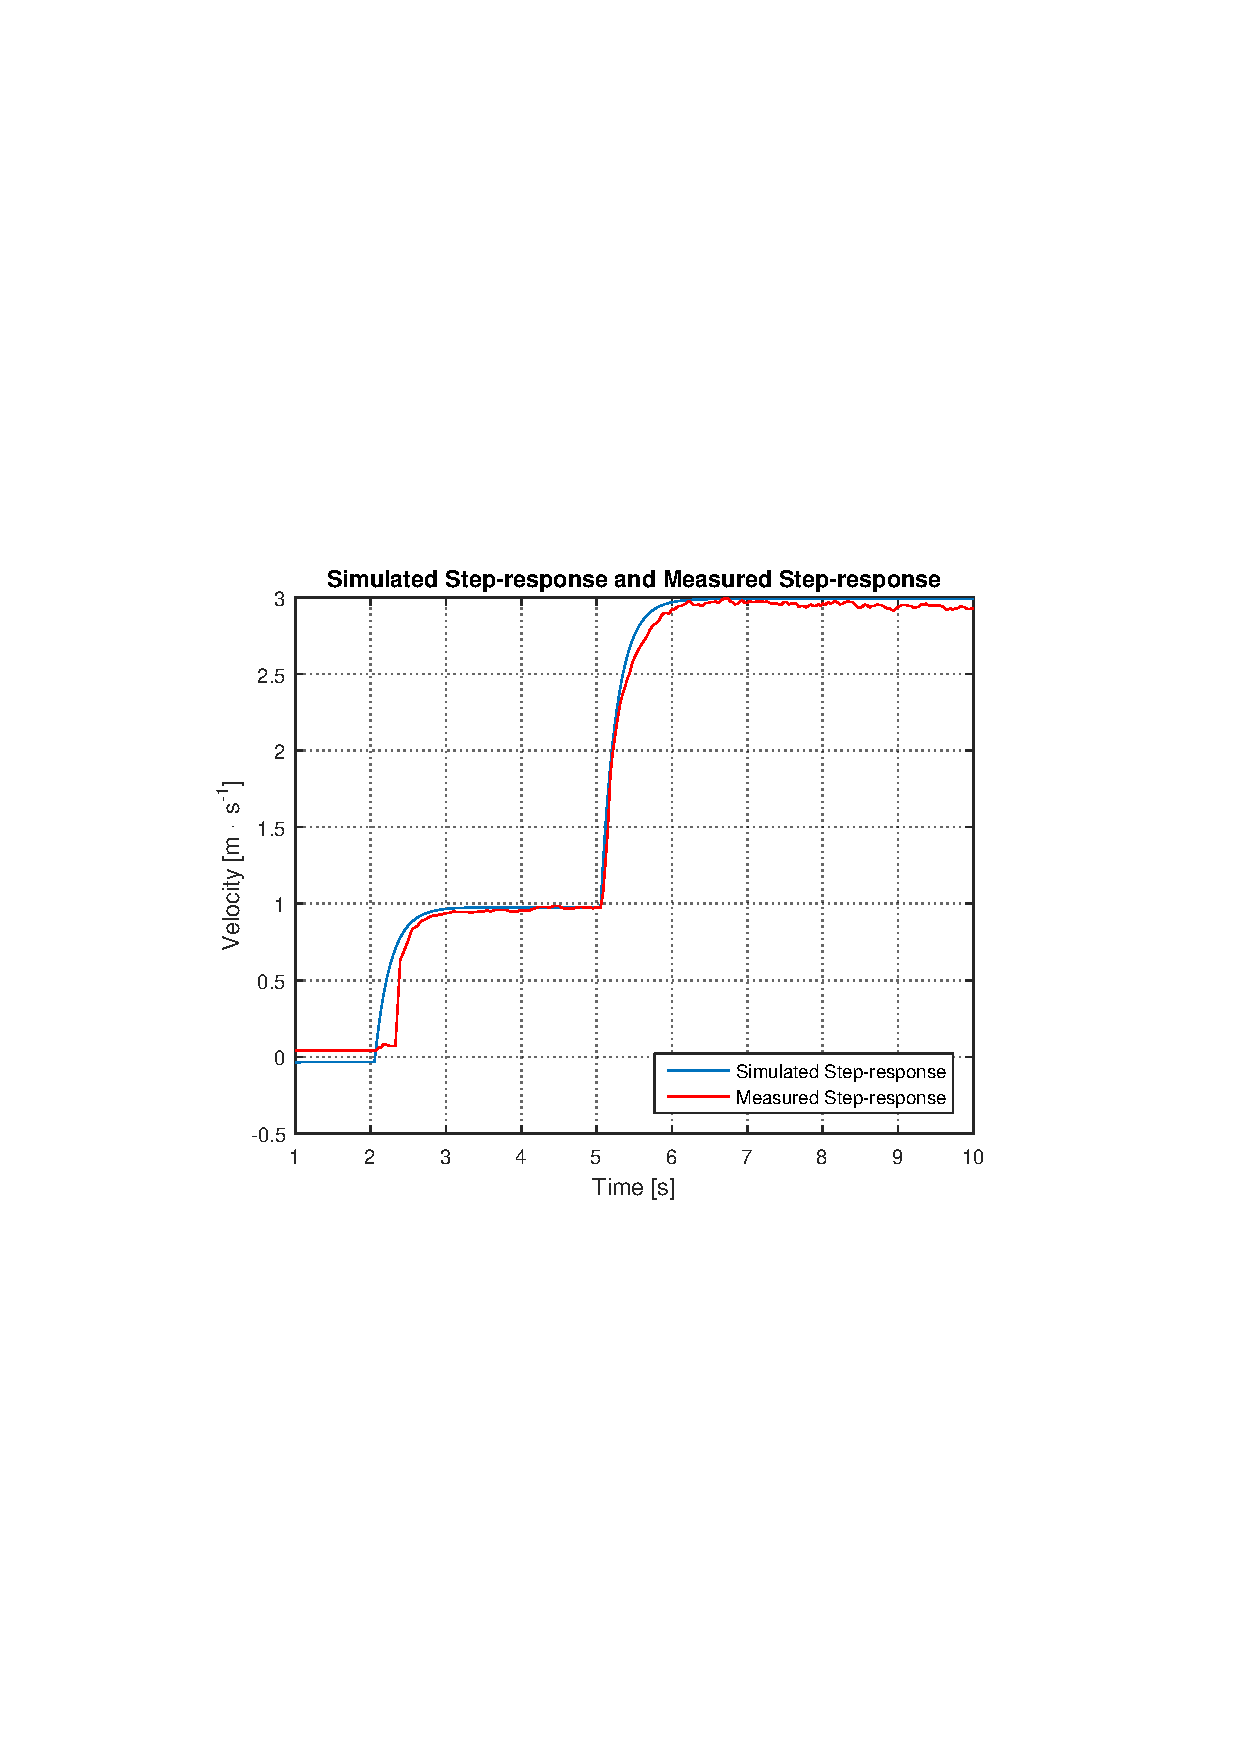
\includegraphics[width=1.4\textwidth]{figures/SimulationIRLsteprespons2.pdf}
  }
  \caption{A plot illustrating a simulated step-response of the approximated velocity model (the blue line) and a measured step-response of the vehicle (the red line).}
  \label{SimulationIRLsteprespons2}
\end{figure}
%
In \figref{SimulationIRLsteprespons2} the red line is the measured data from the vehicle's step-response. To ensure enough data points is registered by the Hall sensor, when performing the step-response of the vehicle, the vehicle is set to drive at \si{1\ m\cdot s^{-1}} at the start of the test. The vehicle preserves this velocity continuously for three seconds, before the vehicle is set to drive at its maximum velocity. The simulation (the blue line) is set to have the same milestones as the measured step-response of the vehicle. Furthermore it can be seen in \figref{SimulationIRLsteprespons2} that the simulation starts before zero, this is due to rounding errors in simulated transfer-function, which is disregarded.

The occurrence of stiction in the start of the simulation and measured step-response, has been eliminated to a certain extent, which makes it insignificant. Furthermore, even though the vehicle is moving at a velocity of $0$ \si{m \cdot s^{-1}}, the velocity is registered to be $0,04$ \si{m \cdot s^{-1}}, see why in \secref{sec:hallFiltering}. 

The little bump in the beginning of the measured step-response, the red line, is caused by the lag of the Hall sensors. This is, however, disregarded. Additionally, the ripples seen on the measured step-response, when the vehicle is at its maximum velocity, could be caused by different kinds of noise factors, e.g:

\begin{itemize}
\item Uneven belts
\item Uneven floor
\item Belts slipping on the floor
\item Wear and tear on the internal gears
\end{itemize}

The data from the simulated and measured step-response illustrated in \figref{SimulationIRLsteprespons2}, when compared is very similar, except for the bump and ripple on the measured data. Besides these two elements the approximated velocity model is sufficient.